\documentclass{exam}
\usepackage{graphicx} % Required for inserting images
\usepackage{amsmath}
\usepackage[left=3cm, right=3cm]{geometry}
\usepackage{multicol}
\usepackage{xcolor}
\usepackage{hyperref}
\usepackage{amssymb}

%\printanswers % If you want to print answers
%\noprintanswers % If you don't want to print answers
% Specifies the way question are displayed:
\qformat{\textbf{Question\thequestion}\quad(\thepoints)\hfill}
\usepackage{color} % defines a new color
\definecolor{SolutionColor}{rgb}{0.8,0.9,1} % light blue
\shadedsolutions % defines the style of the solution environment
% \framedsolutions % defines the style of the solution environment
% Defines the title of the solution environment:
\renewcommand{\solutiontitle}{\noindent\textbf{Solution:}\par\noindent}




\begin{document}

\large{\textbf{Carbon cycle, Math 101}}

Seckin Demirbas, Raphael Kelly, Sven Bachmann, and Peter Harrington

\normalsize
\hrulefill

\



The $CO_2$ concentration in the atmosphere at a particular point on earth follows a cyclic pattern, due to seasonal changes, in particular in the relative proportions of photosynthesis and respiration in plants at different months of the year. In order to explore this cycle, we can decompose the net flux of $CO_2$ as $$\frac{dc}{dt}=i(t)-o(t),$$ where $i(t)$ is the rate of carbon influx into the atmosphere due to respiration and emissions and $o(t)$ is the rate of carbon outflux out of the atmosphere due to photosynthesis. Both are given in $\text{PgC}/\text{year}$ (Petagrams of carbon per year, where 1 petagram = $10^{15}$ grams).
\begin{enumerate}
    \item  Let $a \geq 0$ and $b > a$ represent two different points in time. 
    \begin{enumerate}
            \item \textbf{Describe concisely} the physical quantity that is represented by $\int_a^b i(t)dt$.

      
        
            \item \textbf{Describe concisely} the physical quantity that is represented by $\int_a^b \left(i(t) - o(t)\right)dt$.

         
            \end{enumerate}

    \item Suppose we let the start of the year (January 1st) be time $t=0$ and start measuring the change in $CO_2$ at this time. Assume that $i(t)=25+5 \cos (2 \pi t)$ and that $o(t)=25(1+\cos(2 \pi t - \pi))$.

        \begin{enumerate}
            \item \textbf{Compute the earliest time $T>0$} at which the amount of $CO_2$ in the atmosphere starts decreasing

    

            \item Does the amount of $CO_2$ in the atmosphere  return to its original value? If so, determine the earliest time $t'>0$ at which this occurs.

         
            
        \end{enumerate}


On climatological time scales, the annual oscillations of $CO_2$ discussed above are small compared to the overall increase in carbon. One possible way to determine the overall increase in carbon is by using averages.

    For a function $f(t)$, its average value from $t=a$ to $t=b>a$ is given by
    \[\dfrac{1}{b-a}\int_a^bf(t)\text{d}t.\]

   Below is a plot of the $CO_2$ concentration at Mauna Loa Observatory since 1960. By observation a simple model of the concentration of atmospheric $CO_2$ since 1960 is \[C(t)=310+4 \cos(2\pi t) +1.65 t\] where $t$ is the time in years after 1960 and here $C(t)$ is measured in ppm (parts per million). The long-term trend of rising carbon dioxide levels is driven by human activities.

   \begin{center}
        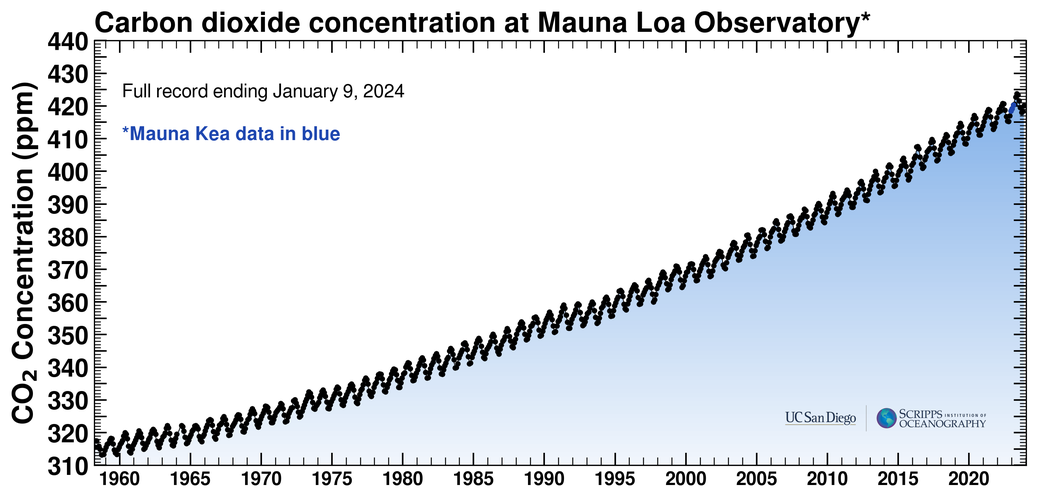
\includegraphics[scale=0.35]{maunaloa2.png}
        
        \textbf{Figure 1.} Graph showing the concentration of atmospheric $CO_2$ since 1960. See \url{https://keelingcurve.ucsd.edu/} for more details
        \end{center}

   Let $A(t)$ be the yearly average of the concentration, namely
\begin{equation*}
    A(t) = \int_t^{t+1}C(s)ds.
\end{equation*}
    \item For $t\in[0,1]$, find the time at which the yearly average is maximal. 



\item Calculate the rate of increase of $A(t)$. That is, how much is the yearly average concentration of atmospheric $CO_2$ increasing per year? 


    

\end{enumerate}

\end{document}
